\section{Benchmark Tabular Domains}
\label{app:domains}

We evaluate on a benchmark of 8 tabular domains, selected for qualitative differences.

\textbf{Gridworlds}. The Gridworld task is an NxN grid with randomly placed walls. The reward is proportional to Manhattan distance to a goal state (1 at the goal, 0 at the initial position), and there is a 5\% chance the agent travels in a different direction than commanded. We vary two parameters: the size ($16 \times 16$ and $64 \times 64$), and the state representations. We use a ``one-hot'' representation, an (X, Y) coordinate tuple (represented as two one-hot vectors), and a ``random'' representation, a vector drawn from $\mathcal{N}(0, 1)^N$, where N is the width or height of the Gridworld. Random observations significantly increase the difficulty, as significant state aliasing occurs.

\textbf{Cliffwalk}: Cliffwalk is a toy example from \citet{Schaul2015}. It consists of a sequence of states, where each state has two allowed actions: advance to the next state or return to the initial state. A reward of 1.0 is obtained when the agent reaches the final state. Observations consist of vectors drawn from $\mathcal{N}(0, 1)^{16}$.

\textbf{InvertedPendulum and MountainCar}: InvertedPendulum and MountainCar are discretized versions of continuous control tasks found in OpenAI gym~\citep{gym}, and are based on problems from classical RL literature. 
In the InvertedPendulum task, an agent must swing up an pendulum and hold it in its upright position. The state consists of the angle and angular velocity of the pendulum. Maximum reward is given when the pendulum is upright. The observation consists of the $\sin$ and $\cos$ of the pendulum angle, and the angular velocity.
In MountainCar, the agent must push a vehicle up a hill, but the hill is steep that the agent must gather momentum by swinging back and forth within a valley to reach the top. The state consists of the position and velocity of the vehicle.

\textbf{SparseGraph}: The SparseGraph environment is a 256-state graph with randomly drawn edges. Each state has two edges, each corresponding to an action. One state is chosen as the goal state, where the agent receives a reward of one.

\iffalse

\section{Fitted Q-iteration with Bounded Projection Error}
\label{app:bounded_error}

When function approximation is introduced to Q-iteration, we lose guarantees that our solution will converge to the optimal solution $Q^*$, because the composition of projection and backup is no longer guaranteed to be a contraction under any norm. However, this does not imply divergence, and in most cases it merely degrades the quality of solution found.

This can be seen by recalling the following result from~\citep{Bertsekas96}, that describes the quality of the solution obtained by fitted Q-iteration (FQI) when the projection error at each step is bounded. The conclusion is that FQI converges to an $\linfnorm$ ball around the optimal solution which scales proportionally with the projection error. While this statement does not claim that divergence cannot occur in general (this theorem can only be applied in retrospect, since we cannot always uniformly bound the projection error at each iteration), it nevertheless offers important intuitions on the behavior of FQI under approximation error. For similar results concerning $\mu$-weighted $\ltwonorm$ norms, see~\citep{munos2005erroravi}.

\begin{theorem}[Bounded error in fitted Q-iteration]
\label{thm:bounded_qi_bound}
Let the projection or Bellman error at each iteration of FQI be uniformly bounded by $\delta$, i.e. $\norm{\hat{Q}_{i+1} - \backup \hat{Q}_i}_\infty \le \delta\ \forall\ i$. Then, the error in the final solution is bounded as

\[  \lim_{i \to \infty} \norm{\hat{Q}_i - Q^*}_\infty \le \frac{\delta}{1-\gamma} \]
\end{theorem}
\begin{proof}
See of Chapter 6 of~\citet{Bertsekas96}.
%Let $\epsilon_i = \norm{\hat{Q}_i - V^*}_\infty$ denote the error at iteration i.
%\begin{align*}
%\epsilon_{i+1} = \norm{\hat{Q}_{i+1} - Q^*}_\infty &= \norm{\hat{Q}_{i+1} -\backup \hat{Q}_i + \backup \hat{Q}_i - Q^*}_\infty \\
%&\le \norm{\hat{Q}_{i+1} -\backup \hat{Q}_i}_\infty + \norm{\backup \hat{Q}_i - Q^*}_\infty \\
%&\le \delta + \gamma\norm{\hat{Q}_i - Q^*}_\infty \\
%&= \delta + \gamma\epsilon_i \\
%\end{align*}
%We have now established a recurrence relationship between $\epsilon_{i+1}$ and $\epsilon_i$. Note that this implies a geometric series:
%\begin{align*}
%\epsilon_{i+1} &\le \delta + \gamma \epsilon_i \\
%&\le \delta + \gamma (\delta + \epsilon_{i-1})\\
%&\cdots \\
%&\le \delta + \gamma \delta + \gamma^2 \delta + \cdots + \gamma^{i+1}\epsilon_0\\
%\end{align*}
%Therefore, since $\gamma<1$, we can apply the limit formula for a geometric series: $\lim_{i \to \infty} \epsilon_i = \lim_{i \to \infty} \sum_{k=0}^i \delta \gamma^k + \gamma^i\epsilon_0= \frac{\delta}{1-\gamma}$. 
\end{proof}

We can use this statement to provide a bound on the performance of the final policy. 

\begin{corollary}
Suppose we run fitted Q-iteration, and let the projection error at each iteration be uniformly bounded by $\delta$, i.e. $\norm{\hat{Q}_{i+1} - \backup \hat{Q}_i}_\infty \le \delta\ \forall\ i$. Letting $\eta(\pi)$ denote the returns of a policy $\pi$, the the performance of the final policy is bounded as:

\[  \lim_{i \to \infty} |\eta(\pi^i) - \eta(\pi^*)| \le \frac{2\gamma\delta}{(1-\gamma)^2} \]
\end{corollary}
\begin{proof}
This result is obtained by substituting Thm.~\ref{thm:bounded_qi_bound} into Propositon 6.1 of ~\citet{Bertsekas96}.
\end{proof}

\subsection{Unbounded divergence in FQI}
\label{app:unbounded_divergence}
Because $\ltwonorm$ norms are bounded by the $\linfnorm$ norm, Thm.~\ref{thm:bounded_qi_bound} implies that \textit{unbounded} divergence is impossible when weighting distribution has positive support at all states and actions (i.e. $\mu(s,a) > 0\ \forall\ (s, a) \in (\mathcal{S}, \mathcal{A})$), and the projection is non-expansive in the $\ltwonorm$ norm (such as when using linear approximators). 

We can bound the $\mu$-weighted $\ltwonorm$ in terms of the $\linfnorm$ as follows: $\normtmu{\cdot} \le \frac{1}{\min \mu(s,a)} \normt{\cdot} \le \frac{\sqrt{|\mathcal{S}||\mathcal{A}|}}{\min \mu(s,a)} \norm{\cdot}_\infty$. Thus, we can apply Thm.~\ref{thm:bounded_qi_bound} with $\delta = \frac{\sqrt{|\mathcal{S}||\mathcal{A}|}}{\min \mu(s,a)}$ to show that unbounded divergence is impossible. Note that because this bound scales with the size of the state and action spaces, it is fairly loose in many practical cases, and practitioners may nevertheless see Q-values grow to large values (tighter bounds concerning L2 norms can be found in \cite{munos2005erroravi}, which depend on the transition distribution). It also suggests that distributions which are fairly uniform (so as to maximize the denominator) can perform well.

When the weighting distribution $\mu$ does not have support over all states and actions, divergence can still occur, as noted in the counterexamples such as Section 11.2 of ~\citet{suttonrlbook}. In this case, we consider two states (state 1 and 2) with feature vectors 1 and 2, respectively, and a linear approximator with parameter $w$. There exists a single action with a deterministic transition from state 1 to state 2, and we only sample the transition from state 1 to state 2 (i.e. $\mu(s,a)$ is 1 for state 1 and 0 for state 2). All rewards are 0. In this case, the projected Bellman backup takes the form:
\[w^{t+1} = \argmin{w} (w - 2\gamma w^t)^2\]
Which will cause unbounded growth $\lim_{t \to \infty} w_t = \infty$ when iterated, provided $\gamma > 0.5$. However, if we add a transition from state 2 back to itself or to state 1, and place nonzero probability on sampling these transitions, divergence can be avoided.

\section{$\alpha$-smoothed Q-iteration}
\label{app:alpha_smoothed_q}

In this section we show that the $\alpha$-smoothed Bellman backup introduced in Section~\ref{sec:analysis_nonstationarity} is still a valid Q-iteration method, in that it is a contraction (for $1 \ge \alpha > 0$) and thus converges to $Q^*$.

We define the $\alpha$-smoothed Bellman backup as:
\[ \backup^{\alpha}Q = \alpha \backup Q + (1-\alpha)Q\]

\begin{theorem}[Contraction rate of the $\alpha$-smoothed Bellman backup]
\label{thm:alpha_smoothed_q}
$\backup^{\alpha}$ is a $1-\alpha+\gamma\alpha$-contraction:
\[ \norm{\backup^{\alpha}Q_1 - \backup^{\alpha}Q_2}_\infty \le (1-\alpha+\gamma\alpha)\norm{Q_1 - Q_2}_\infty\]
\end{theorem}
\begin{proof}
This statement follows from straightforward application of the triangle rule and the fact that $\backup$ is a $\gamma$-contraction:
\begin{align*}
&\norm{\backup^{\alpha}Q_1 - \backup^{\alpha}Q_2}_\infty \\
&= \norm{(\alpha \backup Q_1 - (1-\alpha)Q_1) - (\alpha \backup Q_2 - (1-\alpha)Q_2 }_\infty \\
&= \norm{\alpha (\backup Q_1 - \backup Q_2) + (1-\alpha)(Q_1-Q_2) }_\infty \\
&\le \alpha \norm{\backup Q_1 - \backup Q_2}_\infty + (1-\alpha)\norm{Q_1-Q_2 }_\infty \\
&\le \alpha \gamma \norm{Q_1 - Q_2}_\infty + (1-\alpha)\norm{Q_1-Q_2 }_\infty \\
&=  (1-\alpha + \alpha\gamma) \norm{Q_1 - Q_2}_\infty
\end{align*}
\end{proof}


\begin{figure*}[t!]
\begin{subfigure}[t]{1.0\textwidth}
    \centering
    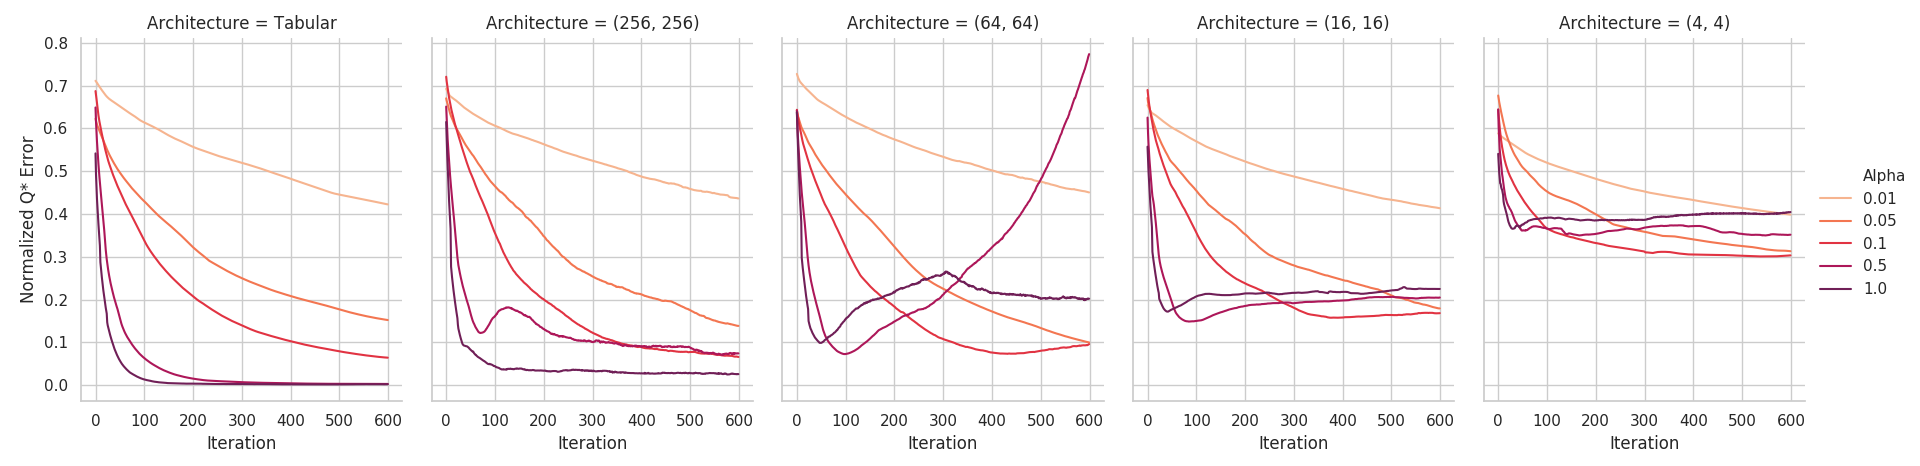
\includegraphics[width=0.99\textwidth]{images/soft_target_qerr}
\end{subfigure}%

\begin{subfigure}[t]{1.0\textwidth}
    \centering
    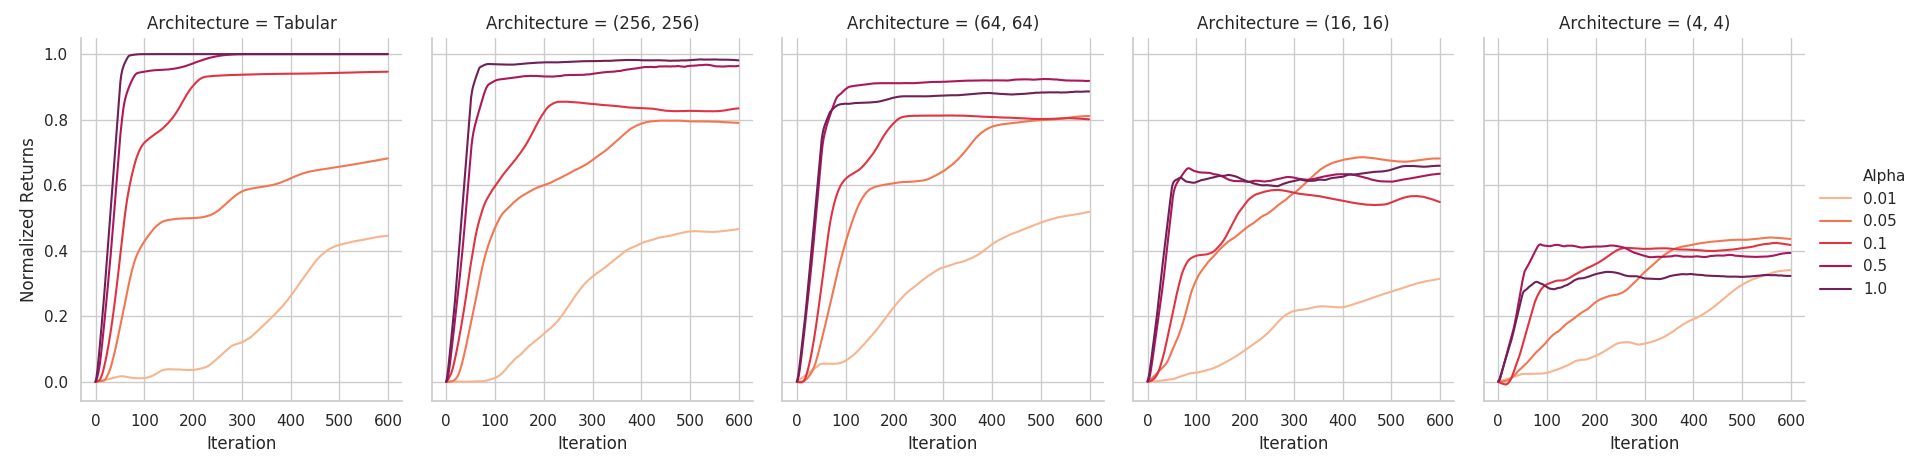
\includegraphics[width=0.99\textwidth]{images/soft_target_returns}
\end{subfigure}%
\caption{\label{fig:smooth_fqi} Results for the $\alpha$-smoothed Bellman backup experiment. Normalized $\linfnorm$ norm error to $Q^*$ and normalized returns plotted for different values of $\alpha$ and architectures. Values are averaged over all domains and 5 seeds. For large architectures, higher values of $\alpha$ result in faster convergence and higher asymptotic returns. However, for smaller architectures, low values of $\alpha$ slightly outperform higher values.}
%script=plot_smoothed_target.py
%data=central1//2019-01-19-newenv-smoothed-target
\end{figure*}

\section{Adversarial Feature Matching (AFM): Detailed Explanation and Practical Implementation}
\label{app:adversarial}
As described in section~\ref{sec:afm}, we devise a novel weighting scheme for the Bellman error objective based on an adversarial minimax game. The adversary computes weights $p_\phi(s, a)$ (representing the weighting distribution $\mu$), for the Bellman error: $(Q_{\theta, w}(s, a) - y(s, a))^2$. Recalling from Section~\ref{sec:afm}, the optimization problem is given by:
\begin{multline*}
    \min_{\theta, w} \max_{\phi} \mathbb{E}_{p_\phi(s, a)} [(Q_{w, \theta} (s, a) - y(s, a))^2]\\
s.t.~~ \big\vert\big\vert \mathbb{E}_{p_\phi(s, a)}[\Phi(s)] - \frac{\sum_i \Phi(s_i)}{N} \vert\vert \leq \varepsilon
\end{multline*}
where $\Phi(s)$ are the state features learned by the Q-function approximator. $\Phi(s)$ is easy to extract out of the multiheaded $Q(s,a)$ ($Q(s, a) = w_a^T\Phi(s)$) model typically used for discrete action control, as one choice is to let $\Phi(s)$ be the output of the penultimate layer of the Q-network. For continuous control tasks, however, we model $\Phi(s, a)$ (which is a function of the actions as well) as state-only features are unavailable, unless separately modeled. This can also be interpreted as modelling a feature matching constraint on the gradient of $Q(s, a)$ with respect to the last linear parameters $w_a$. A possible extension is to take into account the entire gradient as the features in the feature matching constraint, that is, $\nabla_{w, \theta} Q_{w, \theta}(s, a)$.

This choice of the constraint is suitable and can be interpreted in two ways. First, an adversary constrained in this manner has enough power to exploit the Q-network at states which get aliased under the chosen function class, thereby promoting more separable feature learning and reducing some negative aspects of function approximation that can arise in Q-learning. This is also similar in motivation to \citep{martha2018sparse}. Second, this feature constraint also bears a similarity the Maximum Mean Discrepancy (MMD) distance between two distributions $P(x)$ and $Q(x)$ that can be written as $\text{MMD}^2(P, Q) := ||\mathbb{E}_{P}[\Phi] - \mathbb{E}_{Q}[\Phi]||_{\mathcal{H}}$, where the set of functions $\Phi$ is the canonical feature map, $\Phi: \mathbb{R}^n \rightarrow \mathcal{H}$ (from real space to the RKHS). In our context, this is analogous to optimizing a distance between the adversarial distribution $p_\phi(s, a)$ and the replay buffer distribution $p_{rb}(s, a)$ (as the average is a Monte-Carlo estimator of the expected $\Phi$ under the replay buffer distribution $p_{rb}(s, a)$). In the light of these arguments, AFM, and other associated methods that take into account the properties of the function approximator into account (for example, $\Phi$ here), can greatly reduce the bias incurred due to function approximation in the due course of Q-learning/FQI, as depicted in \ref{fig:function_approx}.

\textbf{Comparision to Prioritized Experience Replay (PER): }While both AFM and PER tend to upweight samples in the buffer with a high Bellman error, PER explicitly attempts to \emph{reduce} distribution shift via importance sampling. As we observed in Section~\ref{sec:sampling_distributions}, distributional shift is not actually harmful in practice, and AFM dispenses with this goal, instead explicitly aiming to rebalance the buffer to attain better coverage via adversarial optimization. In our experiments, this results in substantially better performance, consistent with the hypothesis that coverage, rather than reduction of distributional shift, is the most important property in a sampling distribution.

\paragraph{Solving the optimization} We solve this saddle point problem using alternating dual gradient descent. We first solve the inner maximization problem, and then use its solution to then solve the outer minimization problem. We first compute the Lagrangian for the maximization, $\mathcal{L}_{\text{inner}}({\phi; \lambda, \theta})$ by introducing a dual variable $\lambda$,
\begin{multline*}
    \mathcal{L}_{\text{inner}}({\phi; \lambda, \theta}) =  -\mathbb{E}_{p_\phi(s, a)} [(Q_\theta (s, a) - y(s, a))^2] +\\ \lambda \big( \vert\vert \mathbb{E}_{p_\phi(s, a)}[\Phi(s)] - \frac{\sum \Phi(s)}{N} \vert\vert - \varepsilon \big)
\end{multline*}
(Note that this Lagrangian is flipped in sign because we first convert the maximization problem to standard minimization form.) We now solve the inner problem using dual gradient descent. We then plug in the solutions (approximate solutions obtained after gradient descent), $(p^*, \lambda^*)$ into the Lagrangian, to then solve the outside minimization over $\theta$. Note that while $\Phi$  depends on $\theta$ (as it is the feature layer of the Q-network), we don not backpropagate through $\Phi$ while solving the minimization. This improves stability of the Q-network training in practice and to makes sure that Q-function is only affected by FQI updates. In practice, we take up to 10 gradient steps for the inner problem every 1 gradient step of the outer problem. The algorithm is summarized in Algorithm~\ref{alg:afm}. Our results provided in the main paper and here don't particularly assume any other tricks like Optimistic Gradient~\citep{daskalakis2018training}, using exponential moving average of the parameters~\citep{yaz2018the}. Our tabular experiments seemed to benefit some what using these tricks.   

\begin{algorithm}
\caption{\label{alg:afm}AFM with Exact-FQI}
\begin{algorithmic}[1]
    \STATE Initialize Q-value approximator $Q_{\theta, w}(s,a)$, \textbf{projection distribution $\mu_{\phi}(s, a)$, threshold $\varepsilon$}
    \FOR{step $t$ in \{1, \dots, N\}}
    \STATE Initialize Q-value approximator $Q_{\theta, w}(s,a)$.
    \STATE Evaluate $Q_{\theta^t, w^t}(s,a)$ at all states.
    \STATE Compute exact target values at all states. \\
    $y(s,a) = r(s,a) + \gamma E_{s'}[ V_{\theta^t}(s')]$
    \STATE {Minimize the \emph{negative} projection loss with respect to $\phi$ subject to the feature $\Phi$ matching constraint exactly over all states and actions}
    \begin{multline*}
        \phi_{t+1} \leftarrow \arg \min_{\phi} -\mathbb{E}_{p_\phi}[ (Q_{\theta, w}(s, a) - y(s, a))^2] \\
        \text{s.t. } ||\mathbb{E}_{\mu}[\Phi(s, a)] - \frac{\Phi(s, a)}{N}|| \leq \varepsilon\\
    \end{multline*}
    \vspace{-10pt}
    Maximize the Dual Loss w.r.t. $\lambda$.
    \begin{multline*}
        \lambda_{t+1} \leftarrow \arg \max_{\lambda \geq 0} \lambda (||\mathbb{E}_{\mu}[\Phi(s, a)] - \frac{\Phi(s, a)}{N}|| - \varepsilon) 
    \end{multline*}
    \STATE Repeat Step 6 for K steps (K $\in [1, 10]$).
    \STATE Minimize projection loss with respect to $\mu$: \\
    $\theta^{t+1}, w^{t+1} \leftarrow \argmin{\theta, w} E_{p_\phi}[ (Q_{\theta, w}(s,a) - y(s,a))^2]$
    \ENDFOR
\end{algorithmic}
\end{algorithm}

\paragraph{Practical implementation with replay buffers} We incorporate this weighting/sampling distribution into Q-learning in the setting with replay buffers and with state-action sampling. We evaluate the \textbf{weighting version} of our method, AFM, where, we usually sample a large batch $B$ of state-action pairs from a usual replay buffer used in Q-learning, but use importance weights to then match $p_\phi(s,a)$ in expectation. Thus, we use a parametric function approximator to model $\frac{p_\phi(s, a)}{p_{rb}(s, a)}$ -- that is, the importance weights of the adversarial distribution with respect to the replay buffer distribution $p_{rb}(s, a)$. Mathematically, we estimate: $E_{p_\phi(s, a)}[\delta(s, a)] := E_{p_{rb}(s, a)}[\frac{p_\phi(s, a)}{p_{rb}(s, a)} \delta(s, a)]$, where $\delta(s, a) = (Q_{\theta, w} (s, a) - y(s, a))^2$. The latter expectation is then approximated using a set of finite samples. It has been noted in literature that importance sampling (IS) suffers from high variance especially if the number of samples is small. Hence, we use the self-normalized importance sampling estimator, which averages the importance weights in a set of samples or a large number of samples. That is, let $w_{p/p_{rb}} = \frac{p_\phi(s, a)}{p_{rb}(s, a))}$, then instead of using $w_{p/p_{rb}}$ as the importance weights, we use $\Tilde{w}_{p/p_{rb}}(x) = \frac{w_{p/p_{rb}}(x)}{\sum_{y \in B} w_{p/p_{rb}}(y)}$ (where $x$ and $y$ represent state-action tuples; concisely mentioned for visual clarity) as the importance weights. We also regularize the second-order Renyi Divergence between $p_{rb}$ and $p_\phi$ for stability. Mathematically, it can be shown that this is a lower bound on the true expectation of $\delta$ under $p_\phi$, which is being estimated using importance sampling. This result has also been shown in~\citep{metelli2018nips} (Theorem 4.1), where the authors use this lower bound in policy optimization via importance sampling. We state the theorem below for completeness.

\begin{theorem}
\textbf{\citep{metelli2018nips}} Let $P$ and $Q$ be two probability measures on the measurable space $(X , F)$ such that
$P << Q$ and $d_2(P ||Q) < +\infty$. Let $x_1, x_2, \cdots , x_N$ be i.i.d. random variables sampled from $Q$, and $f : X \rightarrow \mathbb{R}$ be a bounded function. Then, for any $0 < \delta \leq 1$ and $N > 0$ with probability at least $1 - \delta$ it holds that:
\begin{multline*}
    \mathbb{E}_{x \sim Q}[f(x)] \geq \frac{1}{N} \sum w_{P/Q}(x_i) f(x_i) -\\ ||f||_{\infty} \sqrt{\frac{(1 - \delta) d_2(P||Q)}{N\delta}}
\end{multline*}
where $d_2(P||Q) \propto \mathbb{E}_{Q} \big[ (\frac{P(x)}{Q(x)})^2 \big]$ is the exponentiated second-order Renyi Divergence between $P$ and $Q$.
\end{theorem}

Hence, our objective for the inner loop now becomes: $ \max_\phi \mathbb{E}_{p_\phi(s, a)} [\delta(s, a)] = \max_\phi \mathbb{E}_{p_{rb}}[\frac{p_\phi(s, a)}{p_{rb}(s, a)} \delta(s, a)]$ is now computed using samples with an additional renyi regularisation term. Since, we end up modeling this ratio,  $f_\phi(s, a) := \frac{p_\theta(s, a)}{p_{rb}(s, a)}$ through out parameteric model, we can hence easily compute an estimator for the Renyi divergence term. The overall lower bound inner maximization problem is:
\begin{multline*}
\max_\phi \frac{1}{N} \sum_{(s, a) \sim p_{rb}}[f_\phi(s, a) (Q_{\theta, w} (s, a) - y(s, a))^2] -\\ C \sqrt{\frac{(1 - \delta) (\frac{\sum f_\phi(s, a))^2}{N})}{N\delta}} \\
\text{s.t.~~} \vert\vert \frac{\sum_{s, a \in p_{rb}}[f_\phi(s, a) \Phi(s)]}{N} - \frac{\sum_{s,a \in p_{rb}} \Phi(s)}{N} \vert\vert  \leq \varepsilon
\end{multline*}

We found that this Renyi penalty helped stabilize training. In practice, we model the importance weights: $f_\phi(s, a)$ as a parametric model with an identical architecture to the Q-network. We use parameter clipping for $f_\phi(s, a)$, where the parameter are clipped to $[-0.1, 0.1]$, analogous to Wasserstein GANs~\citep{pmlr-v70-arjovsky17a}. We also found that self-normalization during importance sampling has a huge practical benefit. Note that as the true $\linfnorm$ norm of the Bellman error is not known, for computing $C$ in the Renyi Divergence term, and hence we either replace it by constant, or compute a stochastic approximation to the $\linfnorm$ norm over the current batch. We found the former to be more stable, and hence, used that in all our experiments. This coefficient of the Renyi divergence penalty is tuned uniformly between $[0.0, 0.25]$. The learning rate for the adversary was chosen to be 1e-4 for the tabular environments, and 5e-4 for TD3. The batch size for our algorithm was chosen to be 128 for the tabular environments and 500 for TD3/SAC. Note that a larger batch size ensures smoothness in the minmax optimization problem. We also found that instead of having a $1D$ Lagrange multiplier for the feature matching constraint, having $d$ Lagrange multipliers for constraining each of the individual dimensions of the features $\Phi \in \mathbb{R}^d$ also helps very much. This is to ensure that the hyperparameters remain the same across different architectures regardless of the dimension of the penultimate layer of the Q-network. The algorithm in this case is exactly the same as the algorithm before with a vector valued dual variable $\lambda$. We used TD3 and SAC implementations from rlkit (\url{https://github.com/vitchyr/rlkit/tree/master/rlkit})

\textbf{Results on MuJoCo Domains: } We find that in all 3 tested domains (Half-Cheetah, Hopper and Ant), AFM yields substantial empirical improvement in the case of TD3 (Fig.~\ref{fig:td3_results_adv}) and performs slightly better than entropy constrained SAC (Fig.~\ref{fig:sac_results_adv}). Surprisingly, we found PER to not work very well in these domains. In light of these results, we conclude that: (1) the choice of sampling distribution is very  important for performance, and (2) considerations such as incorporating knowledge about the function approximator (for example, through $\Phi$) into the choice of $\mu$ (the sampling/weighting distribution) can be very effective.

\begin{figure*}[t]
\begin{subfigure}[t]{0.33\textwidth}
    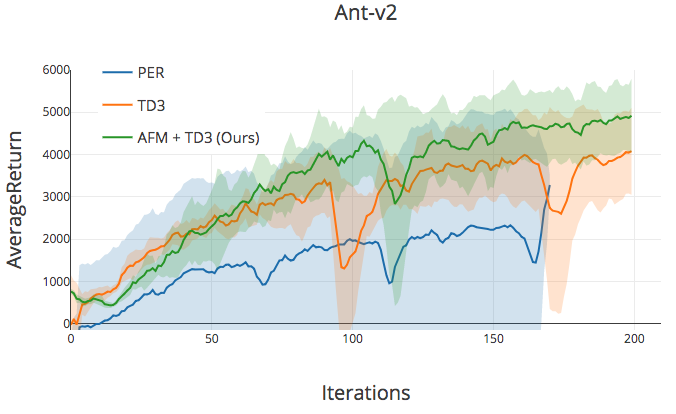
\includegraphics[scale=0.24]{images/ant_td3_final.png}
    \caption{Ant-v2}
\end{subfigure}
\begin{subfigure}[t]{0.33\textwidth}
    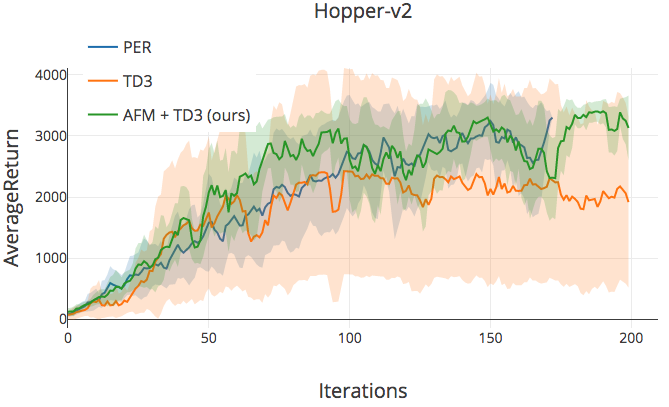
\includegraphics[scale=0.24]{images/hopper_td3_final.png}
    \caption{Hopper-v2}
\end{subfigure}
\begin{subfigure}[t]{0.33\textwidth}
    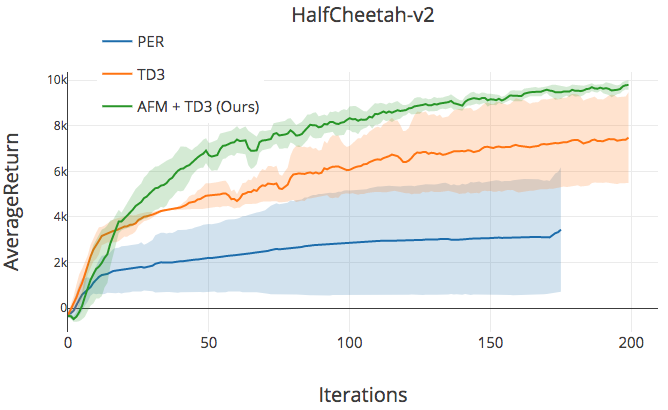
\includegraphics[scale=0.24]{images/cheetah_td3_final_new.png}
    \caption{HalfCheetah-v2}
\end{subfigure}
\caption{Average Return for rollouts performed with a trained the TD3 algorithm with/without \textbf{AFM} (Ours) and with Prioritized Replay (PER). Note that on an average AFM performs better than the baseline and the Prioritized Replay. Each iteration on the x-axis corresponds to 5000 environment steps.}
\label{fig:td3_results_adv}
\end{figure*}

\begin{figure*}[t]
\begin{subfigure}[t]{0.33\textwidth}
    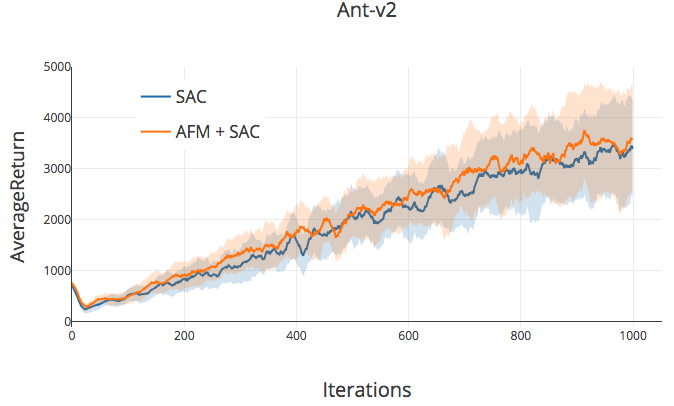
\includegraphics[scale=0.24]{images/ant_sac.png}
    \caption{Ant-v2}
\end{subfigure}
\begin{subfigure}[t]{0.33\textwidth}
    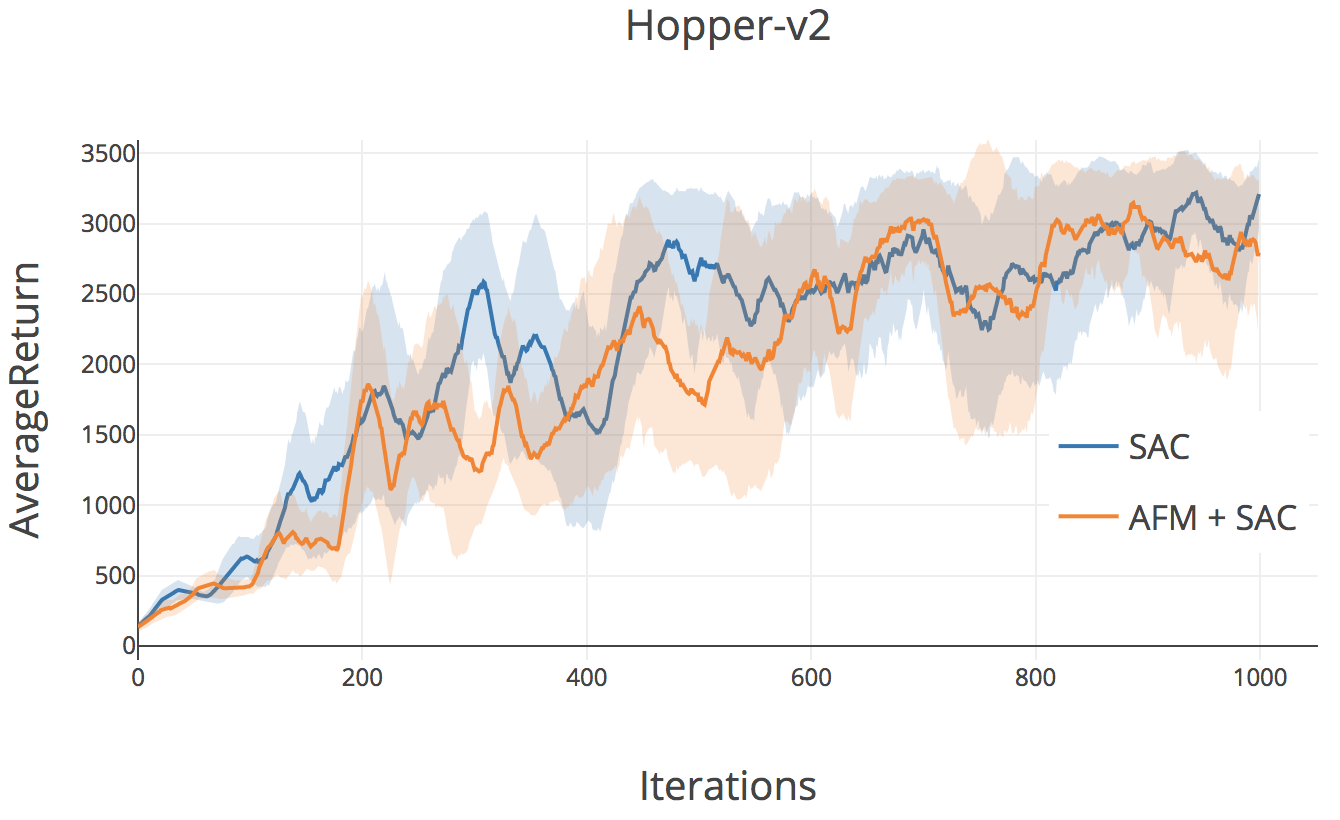
\includegraphics[scale=0.24]{images/hopper_sac.png}
    \caption{Hopper-v2}
\end{subfigure}
\begin{subfigure}[t]{0.33\textwidth}
    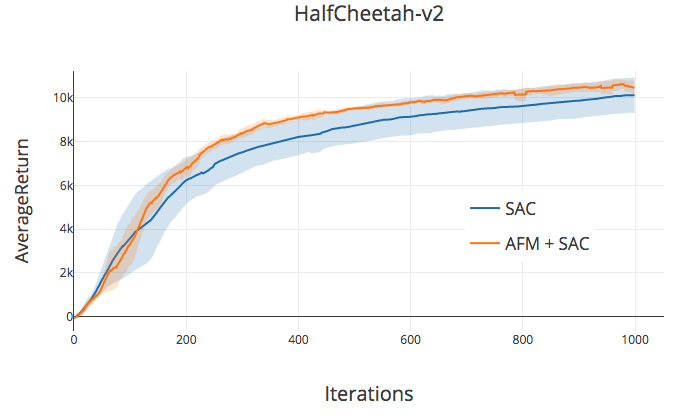
\includegraphics[scale=0.24]{images/cheetah_sac.png}
    \caption{HalfCheetah-v2}
\end{subfigure}
\caption{Average Return for rollouts performed with a trained SAC model with temperature auto-tuning~\citep{haarnoja2018sacapps} with/without AFM. Note that on an average AFM performs slightly better and is always atleast at par with SAC. Each iteration on the x-axis corresponds to 1000 environment steps.}
\label{fig:sac_results_adv}
\end{figure*}

\onecolumn{\section{Function approximation analysis on Mujoco Tasks}}
\label{appendix:sac_size_plots}
As discussed in Section \ref{sec:function_approx}, we validate our findings on the effect of function approximation on 3 MuJoCo tasks from OpenAI Gym with the SAC algorithm from the author's implementation at \cite{haarnoja2018sacapps}. We observe that bigger networks learn faster and better in general.
\begin{figure*}[ht]
    \begin{subfigure}[t]{0.30\textwidth}
        \centering
        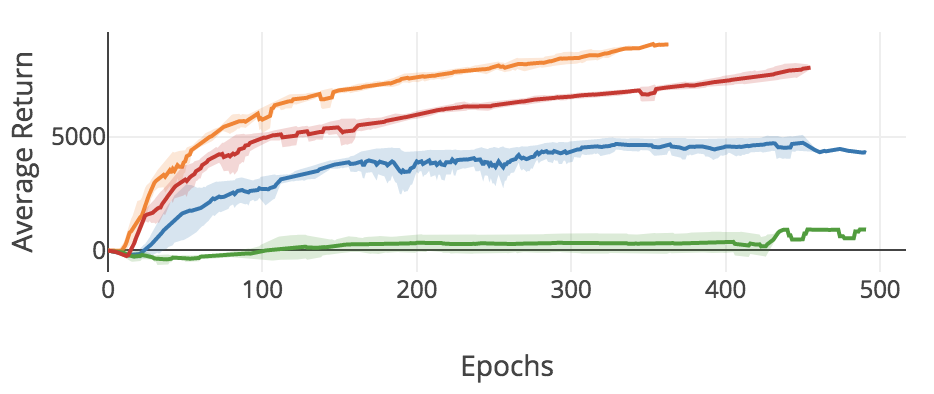
\includegraphics[height=1.2in]{images/cheetah_sizes.png}
        \caption{\centering{HalfCheetah-v2}}
    \end{subfigure}%
    \begin{subfigure}[t]{0.30\textwidth}
        \centering
        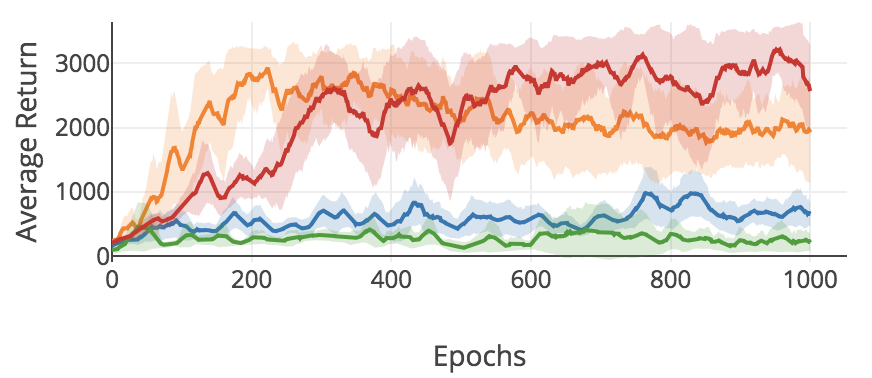
\includegraphics[height=1.2in]{images/hopper_sizes.png}
        \caption{\centering{Hopper-v2}}
    \end{subfigure}
    \begin{subfigure}[t]{0.39\textwidth}
        \centering
        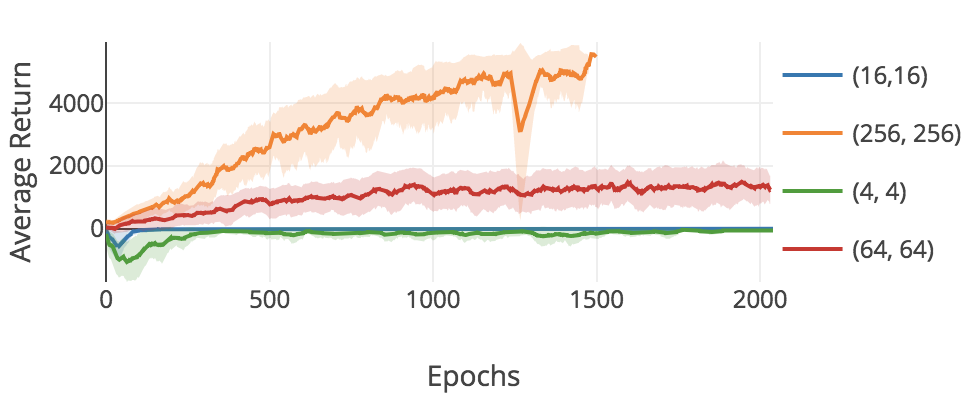
\includegraphics[height=1.2in]{images/ant_sizes.png}
        \caption{\centering{Ant-v2}}
    \end{subfigure}
    \caption{\label{fig:size_sac}Performance of different size architectures on 3 benchmark MuJoco tasks from OpenAI gym suite with the SAC algorithm. Values are averaged over 3 different seeds. A bigger network performs better in terms of learning speed and performance measured in terms of returns. Each epoch on the x-axis corresponds to 1000 environment steps.}
\end{figure*}

% % \subsection{Results with Replay-FQI -- Comparison between PER, Prioritized($s, a$) and AFM}
\section{Additional Plots}

\begin{figure*}[h]
    \centering
    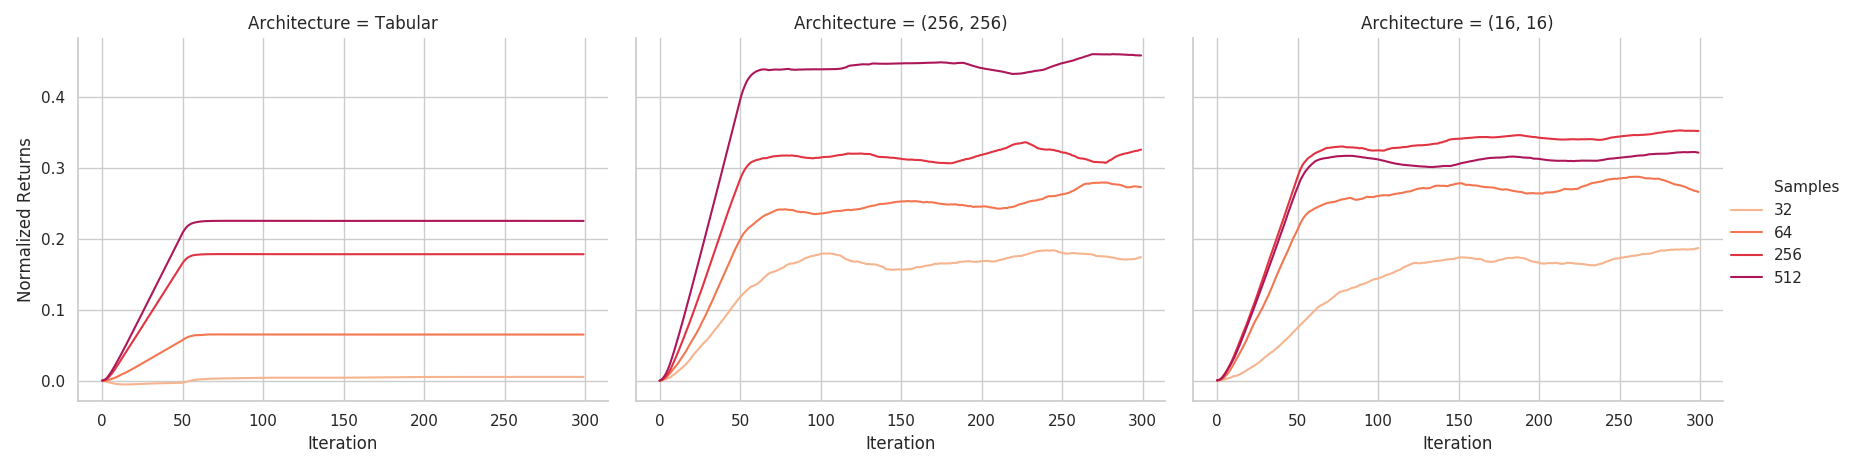
\includegraphics[width=0.99\textwidth]{images/sampling_returns}
\caption{\label{fig:sampling_arch_sweep} Normalized returns with Sampled-FQI, varying over architectures and number of on-policy samples.}
%script=plot_smoothed_target.py
%data=central1//2019-01-19-newenv-smoothed-target
\end{figure*}

\vspace{-30pt}
\begin{figure*}[h]
    \centering
    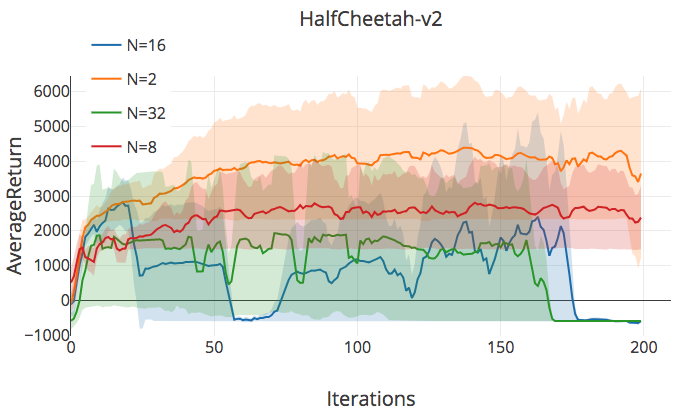
\includegraphics[width=0.49\textwidth, scale=0.25]{images/grad_steps_td3.png}
    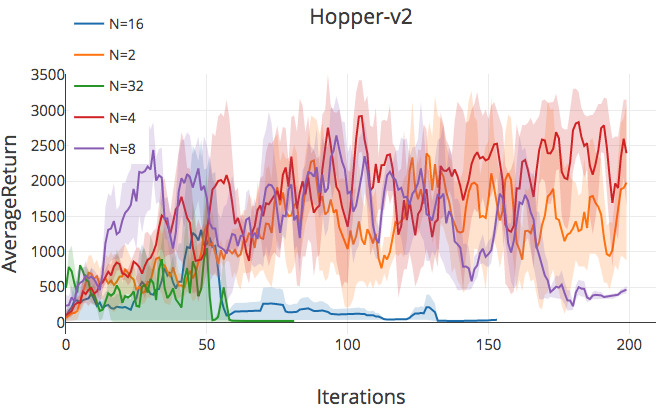
\includegraphics[width=0.49\textwidth, scale=0.25]{images/hopper_grad_steps_td3.png}
\caption{\label{fig:td3_grad_sweep} Performance on Half Cheetah and Hopper trained via TD3 with replay buffer of size $2e4$ with increasing number of gradient steps taken per environment step ($N$) on the critic and the actor. Note the clearly observable decay in performance of the agent with more number of gradient steps -- which clearly validates our claim of the presence of overfitting in Q-functions. Each iteration on the x-axis corresponds to taking 5000 steps in the environment.}

\end{figure*}

\fi